\begin{frame}{Modelo relacional}
    \centering
    \Huge \textcolor{blue3}{Operaciones}
\end{frame}

{
\setbeamertemplate{background} 
{
    
\includegraphics[width=\paperwidth,height=\paperheight]{img/events.jpg}
}
\begin{frame}
\end{frame}
}

\begin{frame}{Un modelo transaccional}
    \begin{block}{Transacciones}
        Una transacci\'on es un \textcolor{red}{conjunto de operaciones que
        modifican el estado de la base de datos} y:

        \begin{itemize}
            \item<2-> \textit{\textcolor{red}{\textbf{\it A}}tomicity}: Se considera como una sola operaci\'on, es decir, se
            realizan todos los cambios o no se realiza ninguno.
            \item<3-> \textit{\textcolor{red}{\textbf{\it C}}onsistency}: El estado de la base de datos es consistente antes y despu\'es de ejecutarse la transacci\'on, pudiendo no serlo durante la ejecuci\'on.
            \item<4-> \textit{\textcolor{red}{\textbf{\it I}}solation}: El estado intermedio de una transacci\'on no
            es visible por el resto de las transacciones: se aisla.
            \item<5-> \textit{\textcolor{red}{\textbf{\it D}}urability}: Luego de ejecutada la transacci\'on, los cambios
            de estado son persistentes y no pueden ser deshechos, incluso, en el caso
            de fallos del sistema.
        \end{itemize}
        
        \onslide<6>{
        \centering
        \Huge \textcolor{red}{Propiedades ACID}
        }
    \end{block}

    \note<3>{@NOTE no se puede acceder al estado durante la ejecuci\'on de una transacci\'on}
\end{frame}

\begin{frame}{Operaciones que modifican el estado}
    \begin{block}<2->{Insertar}
        \begin{enumerate}
            \item Debemos comprobar que todas las metarreglas se cumplan para la tupla que vamos a insertar.
        \end{enumerate}
    \end{block}

    \begin{block}<3->{Eliminar}
        \begin{enumerate}
            \item<4-> No tenemos que comprobar las metarreglas en la tupla que vamos a eliminar pues ya est\'a insertada
        \end{enumerate}
        
    \end{block}
    \vspace{3mm}

    \onslide<5>{
        \centering
         \textcolor{red}{¿Y si eliminamos un valor de llave primaria que es el valor de una llave for\'anea?}
    }
    
\end{frame}



\begin{frame}{Operaciones que modifican el estado}
    \begin{block}{Insertar}
        \begin{enumerate}
            \item Debemos comprobar que todas las metarreglas se cumplan para la tupla que vamos a insertar.
        \end{enumerate}
    \end{block}

    \begin{block}{Eliminar}
        \begin{enumerate}
            \item No tenemos que comprobar las metarreglas en la tupla que vamos a eliminar pues ya est\'a insertada
            \item La relaci\'on debe avisar al resto de las relaciones que un valor de la llave primaria se va a eliminar
            \item<2-> Las relaciones que referencian a la tupla eliminada tienen tres opciones: detener la eliminaci\'on, anular la llave for\'anea o eliminar las tuplas que utilicen dicho valor de llave for\'anea.
        \end{enumerate}
        
    \end{block}
    
\end{frame}


{
\setbeamertemplate{background} 
{
    
\includegraphics[width=\paperwidth,height=\paperheight]{img/delete.jpg}
}
\begin{frame}
\end{frame}
}

\begin{frame}{Operaciones que modifican el estado}
    \begin{block}{Actualizar}
      
    \end{block}

    \onslide<2>{
        \centering
        \textcolor{red}{
        Se puede ver como un proceso de insertar una tupla
        y eliminar una tupla.
        }
    }
\end{frame}

\begin{frame}{Operaciones que modifican el estado}
    \begin{block}{Actualizar}
        \begin{enumerate}
            \item Debemos hacer las comprobaciones pertinentes a la inserci\'on de la tupla modificada.
            \item<2-> Si el valor de la llave primaria se modifica debemos avisar al resto de las relaciones para que actualicen
            la llave for\'anea.
            \item<3-> Realizar una transacci\'on de dos operaciones: \begin{enumerate}
                \item Eliminar la tupla original
                \item Insertar la tupla modificada
            \end{enumerate}
        \end{enumerate}
        
    \end{block}
\end{frame}

\begin{frame}{Operaciones para responder preguntas}
    \begin{block}{\'Algebra relacional}  
    \end{block}

    % @NOTE q el a'lgebra relacional sirve para buscar
\end{frame}


{
\setbeamertemplate{background} 
{
    
\includegraphics[width=\paperwidth,height=\paperheight]{img/flashback.jpg}
}
\begin{frame}
\end{frame}
}


\begin{frame}{Operaciones para responder preguntas}
    \begin{block}{\'Algebra relacional}
        \begin{itemize}
            \item Lenguaje procedimental para el manejo y construcci\'on de relaciones.
            \item Compuesta por operandos (variables y relaciones) y operadores (extensi\'on
            de la Teor\'ia de conjuntos).
            \item Las operaciones del \'algebra relacional manipulan y producen
            relaciones (Propiedad relacional del cierre o clausura).
        \end{itemize}    
    \end{block}

\end{frame}


\begin{frame}{Asignaci\'on $(:=)$}

    La asignaci\'on se utiliza para destinar a una variable
    de relaci\'on el valor que se crea a partir de la aplicaci\'on
    de cualesquiera de las operaciones sobre las relaciones
    existentes.
\end{frame}


\begin{frame}{Renombrar}
    Operaci\'on que no afecta el conjunto de
    tuplas presentes en la relaci\'on sino que modifica
    el esquema de la relaci\'on. En espec\'ifico permite
    cambiar el nombre tanto de los atributos como el de la relaci\'on.
\end{frame}

\begin{frame}{Operaciones de Teor\'ia de conjuntos: Ejemplo}
    \centering
    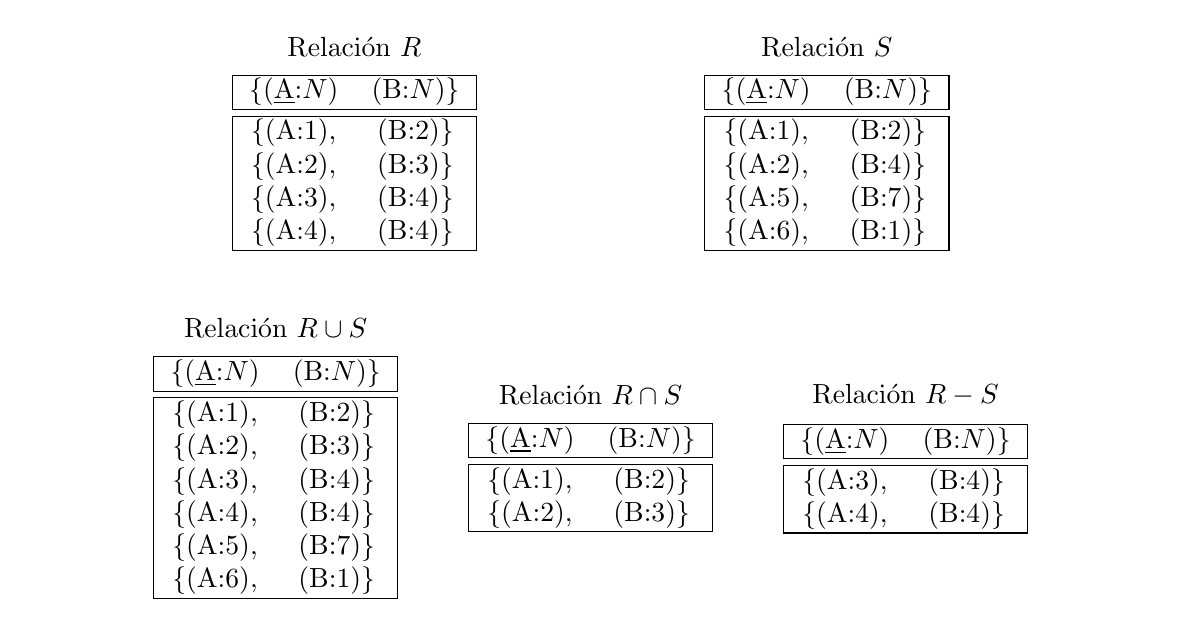
\begin{tikzpicture}
        \node at (0,0) {
            \begin{minipage}{0.50\textwidth}
                \centering
                Relaci\'on $R$\\[2mm]
                \begin{tabular}{|cc|}
                    \hline
                    \{(\underline{A}:$\mathbb{N}$) & (B:$\mathbb{N}$)\}\\
                    \hline
                    \hline
                    \{(A:1), &(B:2)\}\\
                    \{(A:2), &(B:3)\}\\
                    \{(A:3), &(B:4)\}\\
                    \{(A:4), &(B:4)\}\\
                    \hline
                \end{tabular}
            \end{minipage}    
        };

        \node at (6,0) {
            \begin{minipage}{0.50\textwidth}
                \centering
                Relaci\'on $S$\\[2mm]
                \begin{tabular}{|cc|}
                    \hline
                    \{(\underline{A}:$\mathbb{N}$) & (B:$\mathbb{N}$)\}\\
                    \hline
                    \hline
                    \{(A:1), &(B:2)\}\\
                    \{(A:2), &(B:4)\}\\
                    \{(A:5), &(B:7)\}\\
                    \{(A:6), &(B:1)\}\\
                    \hline
                \end{tabular}
            \end{minipage}    
        };

        \node at (-1,-4) {
            \begin{minipage}{0.50\textwidth}
                \centering
                Relaci\'on $R \cup S$\\[2mm]
                \begin{tabular}{|cc|}
                    \hline
                    \{(\underline{A}:$\mathbb{N}$) & (B:$\mathbb{N}$)\}\\
                    \hline
                    \hline
                    \{(A:1), &(B:2)\}\\
                    \{(A:2), &(B:3)\}\\
                    \{(A:3), &(B:4)\}\\
                    \{(A:4), &(B:4)\}\\
                    \{(A:5), &(B:7)\}\\
                    \{(A:6), &(B:1)\}\\
                    \hline
                \end{tabular}
            \end{minipage}    
        };

        \node at (3,-4) {
            \begin{minipage}{0.50\textwidth}
                \centering
                Relaci\'on $R \cap S$\\[2mm]
                \begin{tabular}{|cc|}
                    \hline
                    \{(\underline{A}:$\mathbb{N}$) & (B:$\mathbb{N}$)\}\\
                    \hline
                    \hline
                    \{(A:1), &(B:2)\}\\
                    \{(A:2), &(B:3)\}\\
                    \hline
                \end{tabular}
            \end{minipage}    
        };

        \node at (7,-4) {
            \begin{minipage}{0.50\textwidth}
                \centering
                Relaci\'on $R - S$\\[2mm]
                \begin{tabular}{|cc|}
                    \hline
                    \{(\underline{A}:$\mathbb{N}$) & (B:$\mathbb{N}$)\}\\
                    \hline
                    \hline
                    \{(A:3), &(B:4)\}\\
                    \{(A:4), &(B:4)\}\\
                    \hline
                \end{tabular}
            \end{minipage}    
        };

       

    \end{tikzpicture}

\end{frame}




% \begin{frame}{Intersecci\'on $(R \cap S)$}
%     Dadas dos relaciones $R$ y $S$ con la misma cabecera, la
%     intersecci\'on de dichas relaciones $(R \cap S)$ es una
%     relaci\'on del mismo tipo y con un cuerpo
%     que consiste en todas las tuplas que aparecen tanto en $R$ como en $S$.
% \end{frame}

% \begin{frame}{Diferencia $(R - S)$}
%     Dadas dos relaciones $R$ y $S$ con la misma cabecera, la
%     diferencia de dichas relaciones $(R - S)$ es una
%     relaci\'on del mismo tipo y con un cuerpo
%     que consiste en todas las tuplas que aparecen en $R$ y no en $S$. Esta
%     operaci\'on no es conmutativa.
% \end{frame}


\begin{frame}{Restricci\'on: Ejemplo }
    \centering
    \resizebox{15cm}{!}{
    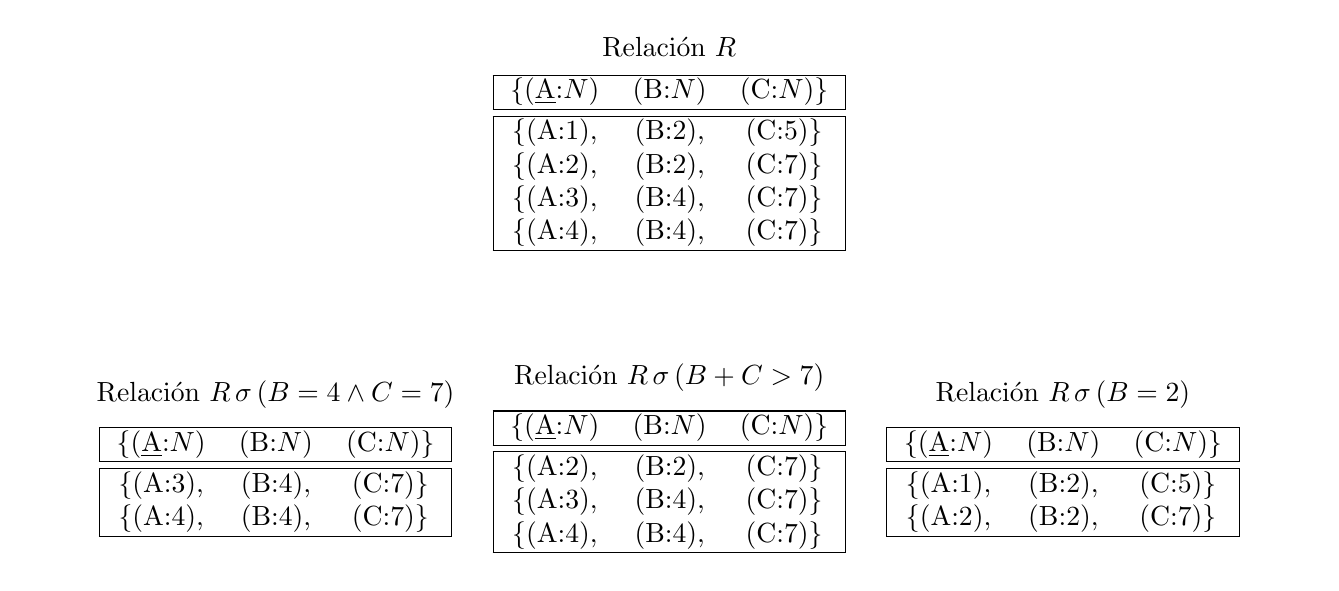
\begin{tikzpicture}
        \node at (0,0) {
            \begin{minipage}{0.50\textwidth}
                \centering
                Relaci\'on $R$\\[2mm]
                \begin{tabular}{|ccc|}
                    \hline
                    \{(\underline{A}:$\mathbb{N}$) & (B:$\mathbb{N}$)  & (C:$\mathbb{N}$)\}\\
                    \hline
                    \hline
                    \{(A:1), &(B:2),  & (C:5)\}\\
                    \{(A:2), &(B:2),  & (C:7)\}\\
                    \{(A:3), &(B:4),  & (C:7)\}\\
                    \{(A:4), &(B:4),  & (C:7)\}\\
                    \hline
                \end{tabular}
            \end{minipage}    
        };

        \node at (5,-4) {
            \begin{minipage}{0.50\textwidth}
                \centering
                Relaci\'on $R \,\sigma\, (B=2)$\\[2mm]
                \begin{tabular}{|ccc|}
                    \hline
                    \{(\underline{A}:$\mathbb{N}$) & (B:$\mathbb{N}$)  & (C:$\mathbb{N}$)\}\\
                    \hline
                    \hline
                    \{(A:1), &(B:2),  & (C:5)\}\\
                    \{(A:2), &(B:2),  & (C:7)\}\\
                    \hline
                \end{tabular}
            \end{minipage}    
        };


        \node at (0,-4) {
            \begin{minipage}{0.50\textwidth}
                \centering
                Relaci\'on $R \,\sigma\,(B + C > 7)$\\[2mm]
                \begin{tabular}{|ccc|}
                    \hline
                    \{(\underline{A}:$\mathbb{N}$) & (B:$\mathbb{N}$)  & (C:$\mathbb{N}$)\}\\
                    \hline
                    \hline
                    \{(A:2), &(B:2),  & (C:7)\}\\
                    \{(A:3), &(B:4),  & (C:7)\}\\
                    \{(A:4), &(B:4),  & (C:7)\}\\
                    \hline
                \end{tabular}
            \end{minipage}    
        };

        \node at (-5,-4) {
            \begin{minipage}{0.50\textwidth}
                \centering
                Relaci\'on $R \,\sigma\, (B =4 \land C=7)$\\[2mm]
                \begin{tabular}{|ccc|}
                    \hline
                    \{(\underline{A}:$\mathbb{N}$) & (B:$\mathbb{N}$)  & (C:$\mathbb{N}$)\}\\
                    \hline
                    \hline
                    \{(A:3), &(B:4),  & (C:7)\}\\
                    \{(A:4), &(B:4),  & (C:7)\}\\
                    \hline
                \end{tabular}
            \end{minipage}    
        };

      

        

       
    \end{tikzpicture}
    }

\end{frame}



\begin{frame}{Proyecci\'on: Ejemplo }
    \centering
    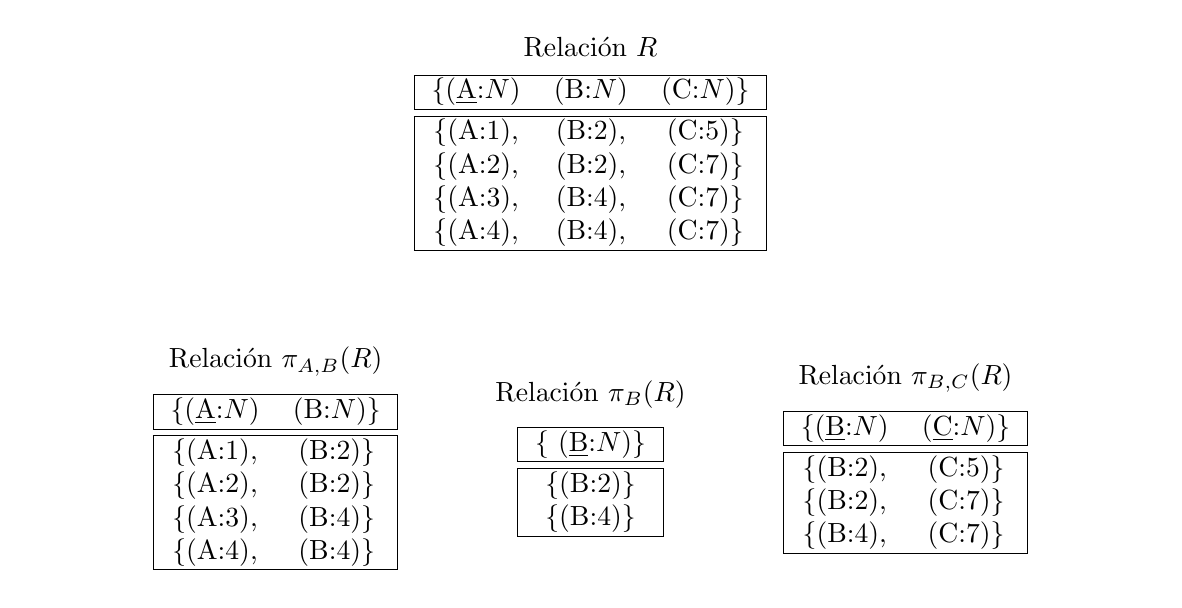
\begin{tikzpicture}
        \node at (0,0) {
            \begin{minipage}{0.50\textwidth}
                \centering
                Relaci\'on $R$\\[2mm]
                \begin{tabular}{|ccc|}
                    \hline
                    \{(\underline{A}:$\mathbb{N}$) & (B:$\mathbb{N}$)  & (C:$\mathbb{N}$)\}\\
                    \hline
                    \hline
                    \{(A:1), &(B:2),  & (C:5)\}\\
                    \{(A:2), &(B:2),  & (C:7)\}\\
                    \{(A:3), &(B:4),  & (C:7)\}\\
                    \{(A:4), &(B:4),  & (C:7)\}\\
                    \hline
                \end{tabular}
            \end{minipage}    
        };

        \node at (-4,-4) {
            \begin{minipage}{0.50\textwidth}
                \centering
                Relaci\'on $\pi_{A,B}(R)$\\[2mm]
                \begin{tabular}{|cc|}
                    \hline
                    \{(\underline{A}:$\mathbb{N}$) & (B:$\mathbb{N}$)\}\\
                    \hline
                    \hline
                    \{(A:1), &(B:2)\}\\
                    \{(A:2), &(B:2)\}\\
                    \{(A:3), &(B:4)\}\\
                    \{(A:4), &(B:4)\}\\
                    \hline
                \end{tabular}
            \end{minipage}    
        };

        \node at (0,-4) {
            \begin{minipage}{0.50\textwidth}
                \centering
                Relaci\'on $\pi_{B}(R)$\\[2mm]
                \begin{tabular}{|c|}
                    \hline
                    \{ (\underline{B}:$\mathbb{N}$)\}\\
                    \hline
                    \hline
                    \{(B:2)\}\\
                    \{(B:4)\}\\
                    \hline
                \end{tabular}
            \end{minipage}    
        };

        \node at (4,-4) {
            \begin{minipage}{0.50\textwidth}
                \centering
                Relaci\'on $\pi_{B,C}(R)$\\[2mm]
                \begin{tabular}{|cc|}
                    \hline
                    \{(\underline{B}:$\mathbb{N}$) & (\underline{C}:$\mathbb{N}$)\}\\
                    \hline
                    \hline
                    \{(B:2), &(C:5)\}\\
                    \{(B:2), &(C:7)\}\\
                    \{(B:4), &(C:7)\}\\
                    \hline
                \end{tabular}
            \end{minipage}    
        };

    \end{tikzpicture}

\end{frame}



\begin{frame}{Producto Cartesiano: Ejemplo}
    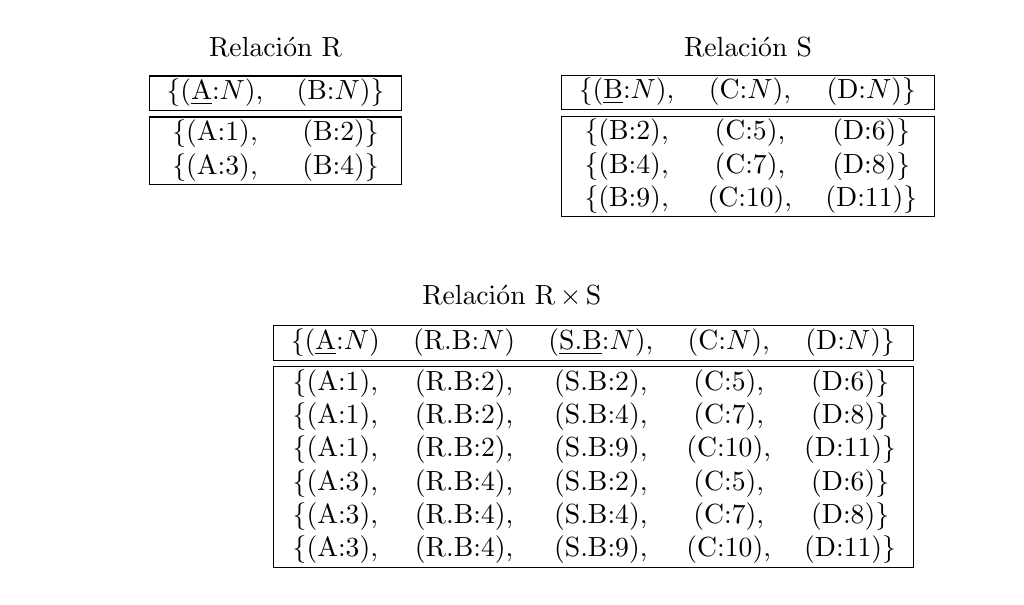
\begin{tikzpicture}
        \node {
            \begin{minipage}{0.50\textwidth}
                \centering
                Relaci\'on R\\[2mm]
                \begin{tabular}{|cc|}
                    \hline
                    \{(\underline{A}:$\mathbb{N}$), & (B:$\mathbb{N}$)\}\\
                    \hline
                    \hline
                    \{(A:1), & (B:2)\}\\
                    \{(A:3), & (B:4)\}\\
                    \hline
                \end{tabular}
            \end{minipage}    
        };


        \node at (6,-0.2) {
            \begin{minipage}{0.50\textwidth}
                \centering
                Relaci\'on S\\[2mm]
                \begin{tabular}{|ccc|}
                    \hline
                    \{(\underline{B}:$\mathbb{N}$), & (C:$\mathbb{N}$), & (D:$\mathbb{N}$)\}\\
                    \hline
                    \hline
                    \{(B:2), & (C:5), & (D:6)\}\\
                    \{(B:4), & (C:7), & (D:8)\}\\
                    \{(B:9), & (C:10), & (D:11)\}\\
                    \hline
                \end{tabular}
            \end{minipage}    
        };

        \onslide<2>{
        \node at (3,-4) {
            \begin{minipage}{0.50\textwidth}
                \centering
                Relaci\'on R$\,\times\,$S\\[2mm]
                \begin{tabular}{|ccccc|}
                    \hline
                    \{(\underline{A}:$\mathbb{N}$) & (R.B:$\mathbb{N}$) & (\underline{S.B}:$\mathbb{N}$), & (C:$\mathbb{N}$), & (D:$\mathbb{N}$)\}\\
                    \hline
                    \hline
                    \{(A:1), &(R.B:2), &(S.B:2), & (C:5), & (D:6)\}\\
                    \{(A:1), &(R.B:2), &(S.B:4), & (C:7), & (D:8)\}\\
                    \{(A:1), &(R.B:2), &(S.B:9), & (C:10), & (D:11)\}\\
                    \{(A:3), &(R.B:4), &(S.B:2), & (C:5), & (D:6)\}\\
                    \{(A:3), &(R.B:4), &(S.B:4), & (C:7), & (D:8)\}\\
                    \{(A:3), &(R.B:4), &(S.B:9), & (C:10), & (D:11)\}\\
                
                    \hline
                \end{tabular}
            \end{minipage}    
        };
        }
    \end{tikzpicture}
\end{frame}





\begin{frame}{Ya tenemos todas las operaciones que necesitamos...}
    \onslide<2>{
    \centering
    \Huge ...para poder definir el resto
    }

\end{frame}


\begin{frame}{Operaciones que combinan relaciones}
    \begin{block}{Natural Join $(R \Join S)$}
        Sean $R$ y $S$ dos relaciones, no necesariamente distintas, distinguimos
        los siguientes conjuntos de atributos:
        \begin{itemize}
            \item El conjunto $R_1,...,R_m$ son atributos de $R$ y no de $S$.
            \item El conjunto $S_1,...,S_n$ son atributos de $S$ y no de $R$.
            \item El conjunto $A_1,...,A_k$ son atributos comunes de $R$ y $S$, es decir, atributos
            con el mismo nombre y mismo dominio asociado en ambas relaciones. 
        \end{itemize}
        La operaci\'on $R \Join S$ \only<2>{\textcolor{red}{($R$ JOIN $S$)} }se define como:\\[2mm]
        \centering
        $
            \pi_{R_1,...,R_m,S_1,...,S_n,R.A_1,...,R.A_k}((R \times S)  \,\sigma\, (R.A_1 = S.A_1 \land ... \land R.A_k = S.A_k))
        $
    \end{block}

    \note<1>{@NOTE insistir en q 2 atributos no son =s si tienen dominios !=s, incluso cuan2 tengan nombres =s}
\end{frame}


\begin{frame}{Natural Join: Ejemplo}
    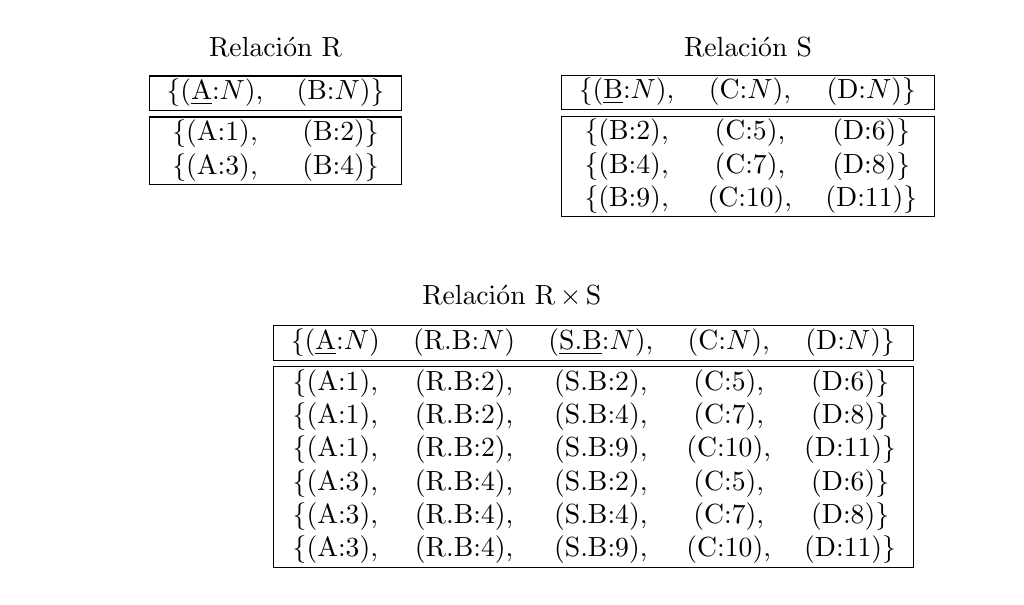
\begin{tikzpicture}
        \node {
            \begin{minipage}{0.50\textwidth}
                \centering
                Relaci\'on R\\[2mm]
                \begin{tabular}{|cc|}
                    \hline
                    \{(\underline{A}:$\mathbb{N}$), & (B:$\mathbb{N}$)\}\\
                    \hline
                    \hline
                    \{(A:1), & (B:2)\}\\
                    \{(A:3), & (B:4)\}\\
                    \hline
                \end{tabular}
            \end{minipage}    
        };


        \node at (6,-0.2) {
            \begin{minipage}{0.50\textwidth}
                \centering
                Relaci\'on S\\[2mm]
                \begin{tabular}{|ccc|}
                    \hline
                    \{(\underline{B}:$\mathbb{N}$), & (C:$\mathbb{N}$), & (D:$\mathbb{N}$)\}\\
                    \hline
                    \hline
                    \{(B:2), & (C:5), & (D:6)\}\\
                    \{(B:4), & (C:7), & (D:8)\}\\
                    \{(B:9), & (C:10), & (D:11)\}\\
                    \hline
                \end{tabular}
            \end{minipage}    
        };


        \node at (3,-4) {
            \begin{minipage}{0.50\textwidth}
                \centering
                Relaci\'on R$\,\times\,$S\\[2mm]
                \begin{tabular}{|ccccc|}
                    \hline
                    \{(\underline{A}:$\mathbb{N}$) & (R.B:$\mathbb{N}$) & (\underline{S.B}:$\mathbb{N}$), & (C:$\mathbb{N}$), & (D:$\mathbb{N}$)\}\\
                    \hline
                    \hline
                    \{(A:1), &(R.B:2), &(S.B:2), & (C:5), & (D:6)\}\\
                    \{(A:1), &(R.B:2), &(S.B:4), & (C:7), & (D:8)\}\\
                    \{(A:1), &(R.B:2), &(S.B:9), & (C:10), & (D:11)\}\\
                    \{(A:3), &(R.B:4), &(S.B:2), & (C:5), & (D:6)\}\\
                    \{(A:3), &(R.B:4), &(S.B:4), & (C:7), & (D:8)\}\\
                    \{(A:3), &(R.B:4), &(S.B:9), & (C:10), & (D:11)\}\\
                
                    \hline
                \end{tabular}
            \end{minipage}    
        };
    \end{tikzpicture}
\end{frame}

\begin{frame}{Natural Join: Ejemplo}
    \centering
    \begin{tikzpicture}
        \node at (0,0) {
            \begin{minipage}{0.50\textwidth}
                \centering
                \onslide<2->{{\color<3>{red}$F: R.B = S.B$}}\\[2mm]

                \centering
                Relaci\'on R$\,\times\,$S\\[2mm]
                \begin{tabular}{|ccccc|}
                    \hline
                    \{(\underline{A}:$\mathbb{N}$) & (R.B:$\mathbb{N}$) & (\underline{S.B}:$\mathbb{N}$), & (C:$\mathbb{N}$), & (D:$\mathbb{N}$)\}\\
                    \hline
                    \hline
                    \{(A:1), &{\color<3>{red}(R.B:2)}, &{\color<3>{red}(S.B:2)}, & (C:5), & (D:6)\}\\
                    \{(A:1), &(R.B:2), &(S.B:4), & (C:7), & (D:8)\}\\
                    \{(A:1), &(R.B:2), &(S.B:9), & (C:10), & (D:11)\}\\
                    \{(A:3), &(R.B:4), &(S.B:2), & (C:5), & (D:6)\}\\
                    \{(A:3), &{\color<3>{red}(R.B:4)}, &{\color<3>{red}(S.B:4)}, & (C:7), & (D:8)\}\\
                    \{(A:3), &(R.B:4), &(S.B:9), & (C:10), & (D:11)\}\\
                
                    \hline
                \end{tabular}
            \end{minipage}    
        };
    \end{tikzpicture}

\end{frame}


\begin{frame}{Natural Join: Ejemplo}
    \centering
    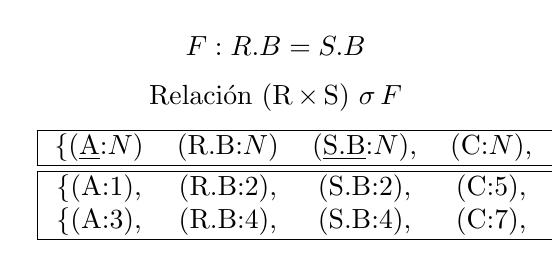
\begin{tikzpicture}
        \node at (0,0) {
            \begin{minipage}{0.50\textwidth}
                \centering
                $F: R.B = S.B$\\[2mm]

                \centering
                Relaci\'on (R$\,\times\,$S) $\sigma\, F$\\[2mm]
                \begin{tabular}{|ccccc|}
                    \hline
                    \{(\underline{A}:$\mathbb{N}$) & (R.B:$\mathbb{N}$) & (\underline{S.B}:$\mathbb{N}$), & (C:$\mathbb{N}$), & (D:$\mathbb{N}$)\}\\
                    \hline
                    \hline
                    \{(A:1), &(R.B:2), &(S.B:2), & (C:5), & (D:6)\}\\
                    \{(A:3), &(R.B:4), &(S.B:4), & (C:7), & (D:8)\}\\
                    \hline
                \end{tabular}
            \end{minipage}    
        };
    \end{tikzpicture}

\end{frame}



\begin{frame}{Natural Join: Ejemplo}
    \centering
    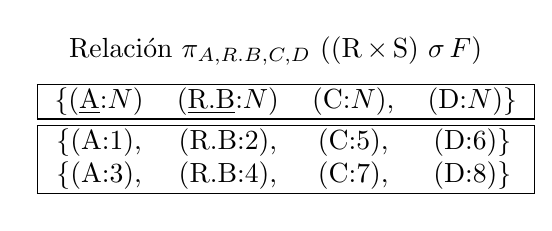
\begin{tikzpicture}
        \node at (0,0) {
            \begin{minipage}{0.50\textwidth}
                \centering
                Relaci\'on $\pi_{A,R.B,C,D}$ ((R$\,\times\,$S) $\sigma\, F$)\\[2mm]
                \begin{tabular}{|cccc|}
                    \hline
                    \{(\underline{A}:$\mathbb{N}$) & (\underline{R.B}:$\mathbb{N}$)  & (C:$\mathbb{N}$), & (D:$\mathbb{N}$)\}\\
                    \hline
                    \hline
                    \{(A:1), &(R.B:2),  & (C:5), & (D:6)\}\\
                    \{(A:3), &(R.B:4),  & (C:7), & (D:8)\}\\
                    \hline
                \end{tabular}
            \end{minipage}    
        };
    \end{tikzpicture}

\end{frame}


\begin{frame}{Natural Join: Ejemplo}
    \centering
    \begin{tikzpicture}
        \node at (0,0) {
            \begin{minipage}{0.50\textwidth}
                \centering
                Relaci\'on R $\Join$ S\\[2mm]
                \begin{tabular}{|cccc|}
                    \hline
                    \{(\underline{A}:$\mathbb{N}$) & (\underline{B}:$\mathbb{N}$)  & (C:$\mathbb{N}$), & (D:$\mathbb{N}$)\}\\
                    \hline
                    \hline
                    \{(A:1), &(B:2),  & (C:5), & (D:6)\}\\
                    \{(A:3), &(B:4),  & (C:7), & (D:8)\}\\
                    \hline
                \end{tabular}
            \end{minipage}    
        };
    \end{tikzpicture}

\end{frame}


\begin{frame}{Operaciones que combinan relaciones}
    \begin{block}{Theta Join ($\theta$-Join)}
        Sean $R$ y $S$ dos relaciones, no necesariamente distintas, definimos el
        $\theta$-Join de $R$ y $S$ como:

        $$
            (R \times S)\,\sigma\, F : F = \theta
        $$  

        donde $\theta$ es un condici\'on, expresada
        mediante una f\'ormula bien formada.
        
    \end{block}
\end{frame}
